%% -*- coding:utf-8 -*-
\documentclass[output=paper
  ,nobabel
  ,uniformtopskip % manual adjustment of pagebreaks
%  ,draftmode
%  ,colorlinks, citecolor=brown
]{langscibook}


\IfFileExists{../localcommands.tex}{%hack to check whether this is being compiled as part of a collection or standalone
   \usepackage{orcidlink}

% add all extra packages you need to load to this file


% Haitao Liu
%\usepackage{xeCJK}
%\setCJKmainfont{SimSun}
%\setCJKmainfont[Scale=MatchUppercase,
%                Path=fonts/
%]{SourceHanSerifSC-Regular}

% instead use option:  ,chinesefont % for references in raffelsiefen.tex
% loading the package changes some spacings


\usepackage{multicol}
\usepackage{tikz}\usetikzlibrary{decorations.pathreplacing}
\usepackage{url}
\urlstyle{same}

%\usepackage{listings}
%\lstset{basicstyle=\ttfamily,tabsize=2,breaklines=true}

\usepackage{langsci-basic}
\usepackage{langsci-optional}
\usepackage[danger]{langsci-lgr}

% toggle danger in texlive 2021
%\newcommand{\M}{\textsc{m}\xspace}

% toggle danger in texlive 2021 or uncomment this
% \newcommand{\N}{\textsc{n}\xspace}
% \newcommand{\F}{\textsc{f}\xspace}


\usepackage{./styles/biblatex-series-number-checks}




\usepackage{langsci-gb4e}




% Demske

\usepackage{tipa}
\usepackage{styles/avm+}
%\usepackage{styles/merkmalstruktur}
\avmfont{\sc}
\usepackage{langsci-forest-setup}
\usepackage{xspace}
%\usepackage{styles/abbrev} 

\usepackage{soul}
\usepackage{color}
\newcommand{\rem}[1]{\textcolor{red}{\st{#1}}}
\newcommand{\add}[1]{\textcolor{blue}{\ul{#1}}}


% Salzmann

\usepackage[nocenter]{qtree}


% Müller

% add this to the default preamble 
\forestset{default preamble={
    for tree={anchor=north},
}}


\usepackage{german}

%\usepackage{german}
\selectlanguage{USenglish}

% Mit Babel geht irgendwie die hyphenation nicht richtig
%\usepackage[ngerman,english]{babel}
%\useshorthands{"} 
%\addto\extrasenglish{\languageshorthands{ngerman}}

\usepackage{styles/makros.2020,
styles/abbrev,
styles/merkmalstruktur,
styles/article-ex,styles/eng-date}


\usepackage{todonotes}
\newcommand{\todostefan}[1]{\todo[color=green!40]{\footnotesize #1}\xspace}
\newcommand{\inlinetodo}[1]{\todo[color=green!40,inline]{\footnotesize #1}\xspace}

\newcommand{\inlinetodoopt}[1]{\todo[color=green!40,inline]{\footnotesize #1}\xspace}
\newcommand{\inlinetodoobl}[1]{\todo[color=red!40,inline]{\footnotesize #1}\xspace}

\newcommand{\itdobl}[1]{\inlinetodoobl{#1}}
\newcommand{\itdopt}[1]{\inlinetodoopt{#1}}

\newcommand{\addpages}{\todostefan{add pages}}

%\newcommand{\iaddpages}{\yel[add pages]{pages}\xspace}



% subfigure
\usepackage{subcaption}



% Nolda
%\usepackage[main=british,nil,german,french]{babel}
\newcommand{\foreignlanguagedummy}[2]{#2}
\usepackage{tagpair}
\usepackage{hang}
\usepackage[noconfig]{ntheorem}
\usepackage{pstricks,pst-node,pst-tree}
\usepackage{newunicodechar}



   \newcommand*{\orcid}[1]{}

% do not show the chapter number. It is redundant, since most references to figures are within the
% same chapter.
\renewcommand{\thefigure}{\arabic{figure}}

\newcommand{\rlapsub}[1]{\rlap{\sub{#1}}}

% \SetupAffiliations{output in groups = false, 
%                    separator between two = {\bigskip\\},
%                    separator between multiple = {\bigskip\\},
%                    separator between final two = {\bigskip\\}
%                    }


%%%%%%%%Alte Umlaute
\newcommand{\oldae}{$\stackrel{\textrm{\tiny e}}{\textrm{a}}$}
\newcommand{\oldoe}{$\stackrel{\textrm{\tiny e}}{\textrm{o}}$}
\newcommand{\oldue}{$\stackrel{\textrm{\tiny e}}{\textrm{u}}$}

\newcommand{\refl}{\REFL}
\newcommand{\pst}{\PST}


% Müller
\let\vref\ref


\let\citew\citet

\newcommand{\page}{}

% biblatex stuff
% get rid of initials for Carl J. Pollard and Carl Pollard in the main text:
\ExecuteBibliographyOptions{uniquename=false}




\newcommand{\nom}{\textsc{nom}}
\newcommand{\gen}{\textsc{gen}}
\newcommand{\dat}{\textsc{dat}}
\newcommand{\acc}{\textsc{acc}}


%\newcommand{\spacebr}{\hspaceThis{[}}



\newcommand{\acknowledgmentsEN}{Acknowledgements}
\newcommand{\acknowledgmentsUS}{Acknowledgments}


% no bf!!!111!
\let\textbfemph\emph

\newcommand{\textbfremoved}[1]{#1}
%\newcommand{\emphremoved}[1]{#1}


\newcommand{\noemph}[1]{#1}
\newcommand{\underlineemph}[1]{\emph{#1}}




% for editing, remove later
\usepackage{xcolor}
\newcommand{\added}[1]{{\red #1}}
\newcommand{\addedthis}{\todostefan{added this}}

\newcommand{\changed}[1]{\textcolor{orange}{#1}}




% Nolda

\theorembodyfont{\normalfont}
\let\restriction\relax
\renewtheoremstyle{break}{\item{\itshape ##1\ ##2}\newline\nopagebreak}{\item{\itshape ##1\ ##2\ (##3)}\newline\nopagebreak}
\theoremstyle{break}
\newtheorem{definition}{Definition}
\newtheorem{pattern}{Pattern}
\newtheorem{restriction}{Restriction}
\newunicodechar{‑}{\hbox{-}}
\newunicodechar{…}{\dots}
\newunicodechar{⁡}{\relax}
\newunicodechar{⁣}{\relax}
\newunicodechar{⁀}{\raisebox{+1ex}{\ensuremath\frown}}
\newunicodechar{⁐}{\raisebox{+1ex}{\ensuremath\frown}\setbox1=\hbox{\ensuremath\smile}\hspace{-\wd1}\raisebox{-1ex}{\ensuremath\smile}}
\newunicodechar{⪪}{\ensuremath{<\mathrel{\llap{\ensuremath{-}}}}}
\setkomafont{descriptionlabel}{\normalfont}
\ExecuteBibliographyOptions{labeldate=comp,labelnumber=true,defernumbers=true}
\defbibenvironment{sources}{\list{\printfield{labelprefix}\,\printfield{labelnumber}}{\settowidth{\labelwidth}{S\,0}\setlength{\labelsep}{\biblabelsep}\setlength{\leftmargin}{\labelwidth}\addtolength{\leftmargin}{\labelsep}\setlength{\itemsep}{\bibitemsep}\setlength{\parsep}{\bibparsep}}\renewcommand{\makelabel}[1]{##1\hfil}}{\endlist}{\item}
\newcommand{\citesource}[1]{\citefield{#1}{labelprefix}\,\citefield{#1}{labelnumber}}


% Was soll das machen?
\newcommand{\textstyleFootnoteSymbol}{}



% Was ist das???? St. Mü. 30.10.2021
%Kann weg. Damit waren die bücker transkripte aligniert. Habe das jetzt mit tabularx und hphantom gemacht

%\newlength{\calength} %tmp length to store the space 1. until [; 2. until ].
%
%%first argument speaker ID, second argument text. Optional argument left margin indicator (arrow or similar)
%\newcommand{\cabox}[3][]{\parbox{0mm}{\hspace*{-1cm}#1}%
%\parbox{1.5cm}{#2}%
%\parbox{9.6cm}{#3}\\%
%}
%
%%translation. First parbox is empty, second parbox takes the translation text
%\newcommand{\trsbox}[1]{\parbox{1.5cm}{~}%
%\parbox{9.6cm}{\itshape #1}\\%
%}
%
%%store the width of a string.
%\newcommand{\settablength}[1]{\settowidth{\calength}{#1}\global\calength=\calength}
%
%%print string and store its width. Useful if the first item of the aligned set is also the longest
%\newcommand{\inittab}[1]{#1\settablength{#1}}
%
%%insert horizontal white space equivalent to the stored width
%\newcommand{\skiptab}{\parbox{\calength}{~}}
%
%%print the argument and fill up with horizontal white space until the stored width is reached.
%\newcommand{\filledtab}[1]{\parbox{\calength}{#1}}



% for standalone compilations Felix: This is in the class already
%\let\thetitle\@title
%\let\theauthor\@author 
\makeatletter
\newcommand{\togglepaper}[1][0]{ 
\bibliography{../bib-abbr,../stmue,../localbibliography,
collection.bib}
  %% hyphenation points for line breaks
%% Normally, automatic hyphenation in LaTeX is very good
%% If a word is mis-hyphenated, add it to this file
%%
%% add information to TeX file before \begin{document} with:
%% %% hyphenation points for line breaks
%% Normally, automatic hyphenation in LaTeX is very good
%% If a word is mis-hyphenated, add it to this file
%%
%% add information to TeX file before \begin{document} with:
%% \include{localhyphenation}
\hyphenation{
Arsch
anaph-o-ra
Bü-cking
con-stit-u-ents
Dor-drecht
For-schungs-ge-mein-schaft
Ge-schich-te
ha-ben
pho-nol-o-gy
pro-so-dic
pro-so-di-cally
Sal-pe-ter
sei-nen
Wil-liams
}
\hyphenation{
Arsch
anaph-o-ra
Bü-cking
con-stit-u-ents
Dor-drecht
For-schungs-ge-mein-schaft
Ge-schich-te
ha-ben
pho-nol-o-gy
pro-so-dic
pro-so-di-cally
Sal-pe-ter
sei-nen
Wil-liams
}
  % \memoizeset{
  %   memo filename prefix={hpsg-handbook.memo.dir/},
  %   % readonly
  % }
  \papernote{\scriptsize\normalfont
    \@author.
    \titleTemp. 
    To appear in: 
    Ulrike Freywald \& Horst Simon (eds.) Headedness and/or grammatical anarchy?
    Berlin: Language Science Press. [preliminary page numbering]
  }
  \pagenumbering{roman}
  \setcounter{chapter}{#1}
  \addtocounter{chapter}{-1}
}
\makeatother



% This does a linebreak for \gll for long sentences leaving space for the language at the right
% margin. The factor .0989 is needed since otherwise starred examples cause a linebreak.
% St.Mü. 17.06.2021 08.02.2021
\newcommand{\longexampleandlanguage}[2]{%
%\begin{tabularx}{.99\linewidth}[t]{@{}X@{}p{\widthof{(#2)}}@{}}%
%\begin{minipage}[t]{.99\linewidth}%
\begin{tabularx}{\linewidth}[t]{@{}X@{}p{\widthof{(#2)}}@{}}%
\begin{minipage}[t]{\linewidth}%
#1%
\end{minipage} & (\ili{#2})%
\end{tabularx}}

% ORCIDs in langsci-affiliations 
\usepackage{orcidlink}
\definecolor{orcidlogocol}{cmyk}{0,0,0,1}
\ProvideDocumentCommand{\LinkToORCIDinAffiliations}{ +m }
  {%
    \orcidlink{#1}
  }

   %% hyphenation points for line breaks
%% Normally, automatic hyphenation in LaTeX is very good
%% If a word is mis-hyphenated, add it to this file
%%
%% add information to TeX file before \begin{document} with:
%% %% hyphenation points for line breaks
%% Normally, automatic hyphenation in LaTeX is very good
%% If a word is mis-hyphenated, add it to this file
%%
%% add information to TeX file before \begin{document} with:
%% %% hyphenation points for line breaks
%% Normally, automatic hyphenation in LaTeX is very good
%% If a word is mis-hyphenated, add it to this file
%%
%% add information to TeX file before \begin{document} with:
%% \include{localhyphenation}
\hyphenation{
Arsch
anaph-o-ra
Bü-cking
con-stit-u-ents
Dor-drecht
For-schungs-ge-mein-schaft
Ge-schich-te
ha-ben
pho-nol-o-gy
pro-so-dic
pro-so-di-cally
Sal-pe-ter
sei-nen
Wil-liams
}
\hyphenation{
Arsch
anaph-o-ra
Bü-cking
con-stit-u-ents
Dor-drecht
For-schungs-ge-mein-schaft
Ge-schich-te
ha-ben
pho-nol-o-gy
pro-so-dic
pro-so-di-cally
Sal-pe-ter
sei-nen
Wil-liams
}
\hyphenation{
Arsch
anaph-o-ra
Bü-cking
con-stit-u-ents
Dor-drecht
For-schungs-ge-mein-schaft
Ge-schich-te
ha-ben
pho-nol-o-gy
pro-so-dic
pro-so-di-cally
Sal-pe-ter
sei-nen
Wil-liams
}
   \togglepaper[9]
}{}

\ChapterDOI{10.5281/zenodo.7142716}


\title{Heads and feet in prosody, poetry, and natural metrics} 

\author{Patrizia {Noel Aziz Hanna}\orcid{0000-0001-7016-8587}\affiliation{Otto-Friedrich-Universität Bamberg}}
% \chapterDOI{} %will be filled in at production

% \epigram{}

\abstract{This paper focuses on three issues concerning headedness vs.\ grammatical anarchy   in German prosody. 1) Language contact: Poetic metres which are designed without metrical heads cannot be   transferred to German without heads. 2) Language change and syntactic structure: German(ic)   anacruses are `headless' structures in terms of prosody – but the result of subsystem   interactions. 3) Theory of metrics: Natural metrics privileges a flat prosodic hierarchy.}


\begin{document}

\maketitle
\section{Poetic metres as long-term experiments of perception}\label{sec-long-term}

Heads and feet in prosody, poetry, and theories of metrics will be investigated in this paper from the perspective of natural metrics. Natural metrics is part of naturalness theory (cf.\ \citealt{Donegan1979}, \citealt{HurchNathan1996}) and takes seriously the evolution of metrical systems as a result of long-term experiments of language perception and production. This implies that metrical systems do not evolve in arbitrary ways but, under default conditions,\footnote{{Metres which are not forced from outside onto the speakers' community but develop over long periods of time only stylise linguistic features which are part of everyday speech (\citealt{Vennemann1995}; cf.\ also \citealt{Miller1902}, \citealt{Allen1973}).} } offer language-based structural features. Within this framework, the question of headedness inevitably leads on to the next question of whether there is independent evidence for internal hierarchies of linguistic structures in traditions of poetic production and reception. The argumentation is not cyclic, because metrical systems change as a consequence of language change (cf.\ \eg  \cite{NoelAzizHanna2008a}).

The evolution of a metrical system is a collective decision of the speaker community about the stylisation of their mother tongue. When foreign poetic patterns are transferred into the native system, the integrated patterns are hypotheses about the foreign linguistic system; they are assumptions about structural properties of that language. A theory of metrics, in contrast to poetic practice, is the scholarly perspective on poetic production, i.e. the abstraction of the mentioned collective knowledge as an interpretation of linguistic output. As a consequence, both poetry and metrical treatises offer insights into linguistic structure.

It will be argued in this paper that the \ili{German} poetic tradition provides evidence for a flat
prosodic hierarchy. In this flat prosodic hierarchy, stressed syllables form the heads of
feet. There are no layers which extend to morphology (\eg `prosodic word') nor to syntax (\eg
`clitic group'); instead, interactions between phonology, syntax, and other linguistic subsystems
are assumed. Three aspects serve to illustrate headedness vs.\ grammatical anarchy:

\begin{sloppypar}
\begin{enumerate}
    \item Language contact: Poetic metres which are designed without metrical heads cannot be transferred to \ili{German} without heads.

    \item Language change and syntactic structure: \ili{German}(ic) anacruses are `headless' structures in terms of prosody – but the result of subsystem interactions.

    \item Theory of metrics: Natural metrics privileges a flat prosodic hierarchy.
\end{enumerate}
\end{sloppypar}

\largerpage
\noindent
The first aspect gives empirical evidence for an approach which takes the relation between feet and stress seriously. The second one provides evidence that anacrusis cannot be dealt with from the perspective of prosody alone. The third aspect explicates the relation between metrical and phonological theories with respect to headedness.

For a theory of metrics, its phonological foundation as well as the headedness of feet are not trivial issues. The question of whether feet belong exclusively to the domain of metrics or to the domain of prosody, or whether they are inherited from prosodic to metrical systems is a matter of debate. Furthermore, there is the question of whether metrics can be handled exclusively within phonology. Theories of metrics have always been dependent on linguistic theory, which is especially evident with respect to the subject of headedness. 

\section{Language contact: prosodic and metrical heads}\label{sec-languagecontact}

In Standard \ili{German} well-formed language rhythm, every syllable is assigned to a foot. This is not an
arbitrary or mere theoretical regulation, as many examples dealt with by prosodic morphology, such
as morphological shortening, show (cf.\ \eg \citealt{LibermanPrince1977}, \citealt{Vennemann1995};
cf.\ also \citealt{DresherLahiri2005} for metrical shortening). The foot implies headedness for
\ili{German} prosody and metrics, i.e. stress.

The relation between prosody and metrics can be demonstrated by the integration of metres without feet\footnote{For another aspect of prosodic integration, consider the incorporation of quantitative Classical metre into non-quantitative \ili{German} metre, cf.\ \eg \citet{Wackernagel1831} and \citet{NoelAzizHanna2008b}.} into stress-based metrical systems. The \ili{French} alexandrine (\ref{ex-frenchalexandrine}) was transferred to the \ili{German} metrical system (\ref{ex-germanalexandrine}).
\eal
\ex\label{ex-frenchalexandrine}
 \ili{French} alexandrine:  ${\sigma}{\sigma}{\sigma}{\sigma}{\sigma}{\sigma}$ ||  ${\sigma}{\sigma}{\sigma}{\sigma}{\sigma}{\sigma}$(${\sigma}$)\\
\gll Je  suis,  mon  cher  ami,    très  heureux    de  te  voir\\
     I  am  my  dear  friend    very  glad    to  you  see\\
\glt (\textit{Asterix et Cleopatra})

\ex\label{ex-germanalexandrine}
 \ili{German} alexandrine (transl. of (\ref{ex-frenchalexandrine})): |x\'{x}|x\'{x}|x\'{x} || x\'{x}|x\'{x}|x\'{x}|(x)\\
\glll Ich  bin,  mein  lieber  Freund,    sehr  glück  lich,  dich  zu  sehen.\\
      |x  \'{x}|  x  \'{x}|x  \'{x}\hspace{25pt}||  x  \'{x} |x  \'{x}|  x  \'{x}|x\\
      I  am  my  dear  friend    very  glad  {}  you  to  see\\
\glt (\textit{Asterix und Kleopatra})
\glt `I am very glad to see you, my dear friend.'
\zl 
%\itdopt{ex anpassen}

\noindent
There are two revealing innovations in the \ili{German} alexandrine: anacrusis (cf.~Section~\ref{sec-anacrusis}) and stress-based feet. The \ili{French} syllable-counting alexandrine originally did not have feet.\footnote{For experiments of syllabic alexandrines in the Netherlands and in Germany cf.\ \citet*[192-197]{Gasparov1996}.} Therefore a product of linguistic imitation like the \ili{German} alexandrine, which clearly is based on feet, provides evidence with respect to prosodic hierarchy in the framework of natural metrics. The \ili{German} alexandrine is an artistic form which represents the \ili{German} language community's implicit knowledge about prosodic headedness, more precisely, the structure of prosodic feet. 

\largerpage
The \ili{French} model is constructed without feet: In the 16th century, the \ili{French} alexandrine consisted of 12 to 13 syllables with a caesura after the 6th syllable \citep[107]{Coenen1998}. The form of the \ili{French} alexandrine has undergone intense discussion (cf.\ \eg \citealt{Bunia2014}, \citealt{Dufter2010}); for its integration into \ili{German}, the relevant question is what was perceived and considered well-formed by its \ili{German} imitators. Obviously, the number of syllables was understood to be an essential feature of the metre, cf.\ the definition in \citealt{Wagenknecht2007} (s.v. Alexandriner; transl. PN):

\begin{quote}
Metre of \ili{French} origin: twelve or thirteen syllables (depending on the male or female ending) with a colon after the sixth syllable. […] Since Opitz, the \ili{German} alexandrine contains six iambs.\footnote{``Versmaß französischer Herkunft: Zwölf- oder Dreizehnsilbler (je nach männlichem oder weiblichem Schluß) mit Kolongrenze nach der sechsten Silbe. [...] Seit Opitz baut sich im Deutschen der Alexandriner aus sechs Jamben auf.''}
\end{quote}

\noindent
Opitz in his poetic treatment \textit{Buch von der Deutschen Poeterey} (1624) perceived the \ili{French} alexandrine as an iambic metre and combined this with syllable counting and caesuras. His imitation became a consensus in the \ili{German} literary tradition. The donor language's `lack of' foot formation was either not understood or considered non-imitable by the users of the target language. The \ili{French} alexandrine was not iambic and, what is more, it did not contain feet at all, cf.\ \citet[229]{Meschonnic1982}:


\begin{quote}
La nuisance du terme \textit{pied} vient de ce qu'il n'y a pas de code métrique, pas de pieds, et, en ce sens, pas de métrique, en français. […] Comme la seule règle métrique, pour l'alexandrin régulier, concerne l'accent à la 6e et à la 12e position, les autres accents sont rythmiques, non métriques. 
\end{quote}

\noindent
This stands in line with \ili{French}, which is not an iambic language but instead – and fitting well the caesuras –~has phrase-final stress (cf.\ \citealt[229]{Meschonnic1982}, \citealt{Kurylowicz1945}, \citealt{JunFougeron2002}). For a native speaker of \ili{German}, however, \ili{French} disyllabic words sound iambic; words in word lists are stressed like one-word sentences, which, because of the phrase-final stress, are interpreted as iambic feet. Trisyllabic \ili{French} words would, of course, result in an anapaestic interpretation; the alexandrine, however, was not stylised as a metre with both binary and ternary feet. The reason may be that, in the 17th century, \ili{German} metricists excluded ternary feet from \ili{German} poetry.\footnote{Ternary feet had unsuccessfully been proposed by August Buchner in his \textit{Anleitung zur Deutschen Poeterey} (1665).} As a consequence, the iambic interpretation of the alexandrine was canonised. 

The linguistic question which poses itself is whether the fact of reading iambs into a metre without feet is indeed language-based. In other words, how likely is the assumption that an integrated metre like the \ili{German} alexandrine does not encode linguistic structures. If what we find is not the consequence of stress-timed \ili{German} rhythm, why is there syllable counting plus feet and not just syllable-counting? Why are the feet of the \ili{German} alexandrine stress-based and not, for instance, mora-based? Why do these feet consist of two syllables instead of, for example, five syllables? The \ili{German} pattern shows the aforementioned non-arbitrary innovations. Thus the \ili{German} iambic alexandrine is an example of fossilised foreign language interference: the \ili{French} syllable-timed metre was interpreted as an iambic one. 

  Integrated metrical patterns reveal implicit linguistic knowledge. Foreign linguistic and also foreign metrical patterns can only be interpreted within the boundaries of actual speakers' linguistic horizons. Poets work within the rhythmic categories of their native tongue. Thus native prosody shines through in integrated metres – in the process of integration, metres borrowed by \ili{German} poets show stress-timed rhythm. Those metres were assessed by sometimes generations of language producers and language recipients. In the \ili{German} literary tradition, only metrical patterns which could both be successfully produced by poets and easily received by listeners in terms of their linguistic well-formedness were canonised. Both conditions were met with the \ili{German} alexandrine. The \ili{German} alexandrine provides independent evidence for the psycholinguistic reality of stress-based feet in \ili{German}. 

\section{Language change: anacrusis}\label{sec-anacrusis}

Metres stylise sentence rhythm, which results from an interaction between phonology and syntax. The stylisation of sentence rhythm in a metrical pattern means that implicit knowledge of not only prosody but also of syntax is encoded. So what does \ili{Germanic} anacrusis reveal about headedness?

The Standard \ili{German} language rhythm is trochaic-dactylic. Nevertheless, the alexandrine, as an
`iambic' metre, fits \ili{German} so well that it was even used as the predominant verse in \ili{German} baroque
drama. The reason for this fit\footnote{According to \citep[294]{HansonKiparsky1996} constraint FIT,
  ``languages select metres in which their entire vocabularies are usable in the greatest variety of
  ways''. The idea of lexical fit is extended in this paper to syntactic fit.} is that unstressed
syllables typically occur at the beginning of \ili{German} sentences. Since the \ili{Germanic} long line is
generally assumed to have been filled by a sentence, anacruses represent beginnings of
sentences. Therefore the monosyllabic unstressed syllables at the beginnings of alexandrine lines
stand in a long tradition of \ili{Germanic} anacrusis, with up to fourteen unstressed
syllables\footnote{\citet*[§216]{Heusler1925} gives as an example of anacrusis (italics) in the
  Old Saxon \textit{Heliand} (\textit{Heliand}, VII, 605.2): \emph{Saga ûs, undar huilicumu he
    sî thesaro} cunneo afôdit [`Tell us of which of these families he sprouted from'].}. 
Limiting the anacrusis to only one unstressed syllable is a specific trait of the alexandrine in the sense of
a strict regulation. The alternative to the scansion of the \ili{German} alexandrine from the beginning of this article (\ref{ex-germanalexandrine}) has trochees plus anacrusis instead of iambs (\ref{ex-germanalexandrine}$'$):

{\exewidth{(1b$'$)}
\begin{exe}
\exp{ex-germanalexandrine}%label didnt 'stick' to exp\label{ex-germanalexandrine2} %1b-nicht2
\ili{German} alexandrine: x|x́x|x́x|x́ || x|x́x|x́x|x́(x)|\\
\gll Ich  bin,  mein  lieber  Freund,           sehr  glück  lich,  dich  zu  sehen.\\
     x|	  x́	x     |x́~x    |x́\hspace{23pt}|| x     |x́     x	    |x́	  x	|x́~x\\
\end{exe}}
%\itdopt{1b', Betonung einfügen}

\noindent
Since the anacrusis forms an unstressed metrical position, prosodic heads are missing there. Yet anacrusis is no counter-evidence to prosodic headedness. The anacrusis does not belong to any measure.\footnote{The endings of lines are often marked and in many cases can be related to the beginnings of the following lines. However, this is not always successful and thus cannot serve as an explanation for the occurrence of anacruses. The first anacrusis of a poem, for instance, could not be subsumed under such a principle. Also, offsetting endings of lines against anacruses would require that the number of syllables in anacruses is kept within a limit defined by the extended foot. Apart from that, offsetting endings of lines against anacruses would disregard the function of marked line endings, which signals the end of the line to the recipient of oral poetry.} With heads of feet being defined as stressed syllables, this is a trivial statement. The question, however, of why there is anacrusis in \ili{Germanic} poetry, and how it is to be accounted for in a theory of metrics, is not a trivial one. While the \ili{Germanic} metrical system is a strictly constrained system, the variation with respect to anacrusis is peculiar. In addition, since there is consensus that \ili{Germanic} metrics is rooted in music (cf.\ \citealt{Hofmann1963}, \citealt{Jammers1964}), which again presupposes isochrony – at least if the singer was musically accompanied by someone else – strong variation of syllable number in the anacruses is unexpected. The complication can be subsumed under two aspects (cf.\ \citealt{NoelAzizHanna2010}):
% {\citet{NoelAzizHanna2013b}.} word lists in turn are one-word sentences and thus marked occurrences.
\begin{enumerate}
    \item  Anacrusis in \ili{Germanic} metres is, as a rule, not obligatory.

    \item The number of syllables in the anacrusis varies considerably.
\end{enumerate}

\noindent
How does anacrusis ranging from one to fourteen syllables fit an aesthetic pattern which also gets by without anacrusis?\footnote{One has to assume with \citet*[§216]{Heusler1925} that poems with long series of syllables in anacrusis were not sung. Nevertheless, the question remains why anacrusis came into existence at all, i.e. what caused the structure at the beginning of lines.} Since there is no foot formation in anacrusis, the answer to why there is no stressed syllable in this position is not a phonological one. The approach presented here assumes a flat prosodic hierarchy, i.e. a prosodic hierarchy which neither extends to morphology nor to syntax. Instead it is proposed that anacrusis is best dealt with by considering interactions between phonology, syntax, and information structure.%
%
\footnote{Syntactic or information-structural influence on metrical structures are rarely investigated. \citet[224]{Hayes1989}, for instance, states: ``I would like to suggest that metrical rules NEVER refer to syntactic bracketing. In other words, syntax has effects in metrics insofar as it determines the phrasings of the Prosodic Hierarchy. [\ldots] Intuitively, the hypothesis states that meter is essentially a phonological phenomenon.''}

The \ili{Germanic} anacrusis represents a syntactic structure already outlined by Kuhn in the 1930s. Kuhn discusses a systematic difference between Proto"=Indo"=European and \ili{Germanic} syntax. Proto"=Indo"=European beginnings of sentences had been described before by \citet{Wackernagel1892}. The \ili{Germanic} structure corresponding to the Proto"=Indo"=European version of Wackernagel's Law means a series of unstressed syllables at the beginnings of sentences. Kuhn's Law transfers Wackernagel's Law to \ili{Germanic} (\citealt{Kuhn1933}: 8; transl. PN):

\begin{quote}
Sentence particles are found in the first drop of the sentence, i.e. in proclitic position either to the first or to the second stressed word.\footnote{``{Die satzpartikeln stehen in der ersten senkung des satzes, in der proklise entweder zu seinem ersten oder zweiten betonten worte.''}}
\end{quote}
\largerpage
\noindent
I suggest that \ili{Germanic} anacrusis resulted from a compromise between conservative versification and
an adaptation to the new state of \ili{Germanic} syntax. \ili{Germanic} anacrusis is a remnant of the transition
from Proto"=Indo"=European to \ili{Germanic} syntax; neither the prestigious Classical \ili{Latin} nor \ili{French} poetry, which strongly influenced \ili{German} literature, share this peculiarity. In Proto"=Indo"=European syntax, specific words occur in second position after the first word, \eg coordinating sentence conjunctions, a set of adverbs, and object pronouns. (\ref{ex-wackernagelslaw}) visualises the transition from Wackernagel's Law in Proto"=Indo"=European to Wackernagel's Law in \ili{Germanic}, using, by way of example, two translations from \ili{Latin} (cf.\ bold elements).

\eal\label{ex-wackernagelslaw}
\ex\label{ex-carmen}
 \ili{Latin} coordinating sentence conjunction\\
\textit{Vivamus mea Lesbia, atque amemus,\\
 rumores\textbf{que} senum severiorum\\
omnes unius aestimemus assis!\\
\textup{(Catull,} Carmen 5)\\} 

\ex\label{ex-mörike}
\ili{German} coordinating sentence conjunction (transl. by Eduard Mörike)\\
\textit{Lass uns leben, mein Mädchen, und uns lieben,\\
\textbf{Und} der mürrischen Alten üble Reden\\
 Auch nicht höher als einen Pfennig achten.\\}
\ex\label{ex-englishconj}
\ili{English} coordinating sentence conjunction (transl. by Thomas Campion)\\
\textit{My sweetest Lesbia, let us live and love;\\
 \textbf{And} though the sager sort our deeds reprove,\\
 Let us not weigh them. \\}
\zl

\noindent
In (\ref{ex-carmen}), the enclitic \ili{Latin} sentence conjunction occurs in second position. The \ili{German}
(\ref{ex-mörike}) and \ili{English} (\ref{ex-englishconj}) translations, in contrast, show the
corresponding conjunction in first position. Most Wackernagel elements occur regularly in first
position in \ili{Germanic}, with the exception of \ili{Gothic}. They can also occur before the second stressed
word, because the Wackernagel chain can be interrupted, \eg by the finite verb. 

Initial position of Wackernagel elements corresponds to anacrusis in \ili{Germanic} metrics. By contrast, in languages with second-position placement of these elements – i.e. the position originally described by Wackernagel – the chance of sequences of unstressed words at the beginnings sentences is low. \ili{Gothic}, as the oldest attested \ili{Germanic} language, shows characteristics which are similar to Proto"=Indo"=European syntax; for example, its enclitic coordinating sentence conjunction -\textit{uh} `and' occurred in second position.%
%
\footnote{cf.\ Wackernagel's Law in Krisch's presentation \citep[283--284]{Krisch1997}:
\begin{enumerate}
	\item \#X(E)...........\#  \\ X = one word (default)\\ 
	E = Wackernagel enclitic  
\item \#X(E$_1$)C(E$_2$).....\#  \\ 
      E$_1$ and E$_2$ = Wackernagel enclitics \\ 
      E$_1$ = enclitic coordinating conjunctions \\       
      E$_2$ = sentence particles and enclitic pronouns \\ 
      C = subordinating conjunctions, relative pronouns, question pronouns, verbs
\end{enumerate} 
}

\largerpage[2]
If the \ili{Germanic} alliterative verse had its roots in a language with a syntax similar to \ili{Gothic}, the complication of \ili{Germanic} anacrusis would not have occurred at first. The change of Proto"=Indo"=European Wackernagel syntax to the \ili{Germanic} variant of Wackernagel syntax meant a considerable increase of elements in the left sentence periphery before the first stressed content word (cf.\ \figref{figure1}; for details cf.\ \citealt{NoelAzizHanna2015}). The high number of syllables in \ili{Germanic} anacrusis is the result of language change.

\begin{figure}
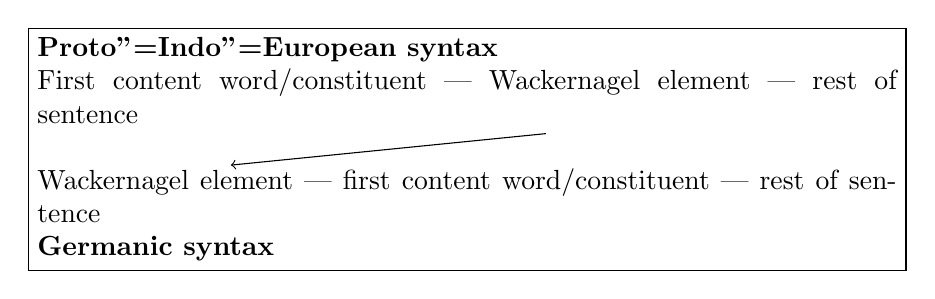
\begin{tikzpicture}
	\node(box)[rectangle,draw]{%
		\begin{minipage}{0.9\textwidth}
			\textbf{Proto"=Indo"=European syntax}\\
			First content word/constituent | Wackernagel element | rest of sentence
			\\
			
			Wackernagel element | first content word/constituent | rest of sentence
			\\
			\textbf{\ili{Germanic} syntax}
		\end{minipage}
	};
	\draw [->] (1,0.2) -- (-3,-0.2);
\end{tikzpicture}	
\caption{The change from Proto"=Indo"=European to Germanic beginnings of sentences} \label{figure1}
\end{figure}

In alliterative verse, the first rhematic word, i.e. usually the first content word, alliterates. Wackernagel's Law does not encompass elements prone to rhematicity, which is why Wackernagel elements usually do not alliterate. Although the syntax had changed, the metrical system at first remained conservative: The `new' unstressed syllables at the beginnings of sentences were not integrated rhythmically into the line, because the principle of assigning the stave to the first rhematic word still prevailed.\footnote{As literary history shows, this principle of versification was given up with time. There are no long sequences of syllables in anacrusis any more. In early Middle High \ili{German}, however, trisyllabic anacrusis is still frequent, and anacrusis with five to six syllables can occur (\citet[§53]{PaulGlier1961}. In the \textit{Nibelungenlied}, disyllabic anacrusis is still possible \citep[37]{Reichert2005}. Despite the prestigious \ili{Romance} ideal of syllable-counting poetry, variation in the anacrusis was upheld as a principle. In the late Minnesang, anacrusis became more and more regulated.} 

\largerpage[2]
Is the \ili{Germanic} anacrusis a headless position? The above argumentation demands a syntactic perspective on the structure. In order to investigate the serialisation principles within the \ili{German} Wackernagel chain, a corpus analysis (1.900.000 words, 190.000 sentences from different genres and regions, starting from Old High \ili{German})\footnote{I am grateful to the IT-Group of the LMU Munich, especially to Christian Riepl, for their indispensable help in programming the SQL database.} was carried out (for details see \citealt{NoelAzizHanna2015}). (\ref{ex-scopalserialisation}) with the Wackernagel chain \textit{endi – auur} gives an example of two adjacent Old High \ili{German} Wackernagel elements. Elements which interrupt the Wackernagel chain (\eg finite verbs or prefields) were skipped, cf.\ (\ref{ex-interrupted}) with the Wackernagel chain: \textit{endi – auur – ni}.

\ea Scopal serialisation (Wackernagel elements underlined)
\ea\label{ex-scopalserialisation}
\gll \underline{Endi}	\underline{auur}	ist	auh	chiscriban:\\ 
and	but	is	also written.\textsc{pii}  \\ 
\glt `And then it is also written:' (Althochdeutscher Isidor, IV, 11)\\

\hspace{-1.5em}Interrupted chain\\
\ex\label{ex-interrupted} 
\gll \underline{Endi}	so	ir	\underline{auur}	dhuo	\underline{ni}	uuas	huuerfandi	zi	dhes ęrrin		meghines		uueghe. \\
and	so	he	but	there	not	was	come.back.\textsc{pi}	to	the former.\textsc{gen.sg}	virtue.\textsc{gen.sg}	way.\textsc{dat.sg}   \\
\glt `And so he did not get back there to the way of virtue.' (Althochdeutscher Isidor XXIX, 11–13)
\z
\z
%\itdopt{anpassen, underline hinzufügen}

\noindent
The corpus, in combination with the \ili{Gothic} evidence, revealed the exceptionless order of elements
presented in \figref{fig2}.\footnote{%
As has been noted above, the chain does not contain rhematic elements. Topicalised negation particles as well as topicalised object pronouns are excluded.}

\begin{figure}
\begin{tabularx}{\textwidth}{|*{5}{>{\centering\arraybackslash}X|}}
	\hline
	 Coordinating sentence conjunctions &  Sentence mood markers &  adverbial connectors &  sentence negation &  object pronouns \\
	\hline
\end{tabularx}
	\caption{Preferred serialisation in the Wackernagel chain}\label{fig2}
\end{figure}

%\itdopt{figure 2 + fußnote einfügen}

The serialisation within the Wackernagel chain follows the scope of elements. Coordinating sentence conjunctions precede sentence mood markers which precede adverbial connectors followed by sentence negation and then object pronouns. Scope decreases from left to right in the chain; it causes the default serialisation within the chain.\footnote{Coordinating sentence conjunctions refer to two sentences and thus have the widest possible scope. Following sentence mood markers, such as the \ili{Gothic} question particle -\textit{u} (cf.\ \citealp{NoelAzizHanna2013a} for its placement), signal the status of the sequence of words as a sentence by fixing its mood; consequently, these markers are the highest heads of the sentence after coordinating sentence conjunctions. Then follow adverbial connectors and the sentence negation in Wackernagel position; adverbial connectors like \ili{German} \textit{nämlich} `namely' cannot be negated. When seen in the light of scopal serialisation, enclitic pronouns have the narrowest scope in the Wackernagel chain. As an ordering principle, scope has already been proposed for \ili{Hittite} (\cite{Luraghi1990}).}  

Scopal serialisation regulates the organisation of sentence beginnings; clearly neither this principle which regulates the relative position of elements in anacrusis nor the information-structural selection of elements in anacrusis are subject to phonology. Unstressedness in anacrusis is derivable because the involved elements are non-rhematic, contributing to discourse organisation, coherence, and cohesion. Thus, although the effect is stresslessness, its motivation lies in information structure.

\section{Natural metrics: privileging a flat prosodic hierarchy}\label{sec-natmetrics} 

Both phonological theories and theories of metrics differ substantially with respect to the concept of headedness. There are, for instance, theories of metrics based on multi-layered prosodic hierarchies\footnote{I.e. in contrast to a flat prosodic hierarchy, which does not extend to morphology or syntax.} which rely on phonology only and theories of metrics which regard feet without relation to speech rhythm. The relation between head and foot is another controversial issue, both in metrics and phonology; the phonological foot plays a major role in theories of metrics, even if a relation between head and foot is rejected. Metrical terminology transports all sorts of theoretical preconditions; differences in concepts of metrical headedness transport conflicting ideas of prosodic hierarchies. 

For illustration, iambicity has been interpreted non-perceptually. \citet*[167;170]{FabbHalle2009} describe the \ili{French} alexandrine – as well as all other \ili{French} syllable counting metres – as iambic: 

\begin{quote}
All \ili{French} meters are in fact organized into iambic feet. […] The grid is not a record of the line that we produce or hear.
\end{quote}

\noindent
\citet*[171]{FabbHalle2009} aim at the representation of their knowledge about the metrical form of a line and note that their approach hightens ``the aesthetic pleasure that competent readers derive from reading verse''. This approach shows an iambic interpretation which differs strikingly from the iambic interpretation of both poets and metricists presented in the sections above. Though it is based on headedness, the concept is not linked to the perception or production of linguistic rhythm. 

The metrical approach of \citet[221]{Hayes1989} points to another direction, representing a synchronic categorisation of metrical production: ``Metrics can be defined as the study of how conventionalized rhythmic patterns are manifested in linguistic material''. Being grounded on multi-layered phonology and stressing parallelisms between metrical and prosodic hierarchies, metrics remains within the field of phonology. With respect to anacrusis, \citet[256-257]{Hayes1989} describes the beginnings of lines as ``extra freedom'':

\begin{quote}
It may be that the principle [``beginnings free, endings strict''] must be accepted as a basic postulate of metrics, unless it follows from deeper psychological principles unknown to me.
\end{quote}

\noindent
While natural metrics shares with Hayes' theory the close orientation to the linguistic material, it
differs from it with respect to the role of linguistic subsystems other than prosody. 

Among the phonological theories which criticise multi-layered phonological hierarchies is the approach of \citet[439;440–441]{HalleIdsardi1995}:

\begin{quote}
We deny the hypothesis that units of prosody are strictly layered in a hierarchy. […] In our framework, the foot is not a theoretical primitive. Rather, metrical boundaries are placed among the stress-bearing elements. In this way, the sequence of stress-bearing elements is subdivided into constituents of various kinds, including iambs and trochees, although iambs and trochees have no privileged status. 
\end{quote}

\noindent
Subsequently, the relation between head and foot has at times been called into question. For
instance, \citet[313]{Hyde2002}, in an OT analysis of binary stress systems, proposes that feet can
overlap, making the foot-stress relationship violable and ``allowing feet to remain stressless under
appropriate rankings''. Similarly, the common structure of poetic and phonological feet has been questioned: ``Poetic feet are constituents, and they can be aligned to
stress positions, but they have no heads'' \citep[1]{VanOostendorp2017}; accordingly, poetic feet
exist just in the interface with phonology since they have no ontology of their own
\citep[11]{VanOostendorp2017}. 

The different conceptions of theories of metrics demonstrate that phonological theory is directly
transferred to theories of metrics. As a matter of course, this is also the case with natural
metrics. Natural phonology neither fits the idea of non-perceptual metrics\footnote{An anonymous
  referee notes: ``I take it that metrics is by definition abstract knowledge of poetic forms, and
  therefore, by its very nature, non-perceptual.'' Literary history documents how this knowledge was
  arrived at; the genre of poetics provides evidence for a perceptual basis of metrics. To give an
  example, \citeauthor{Voss1802}, with his poetics \emph{Zeitmessung} [The measuring of time]
  (\citeyear{Voss1802}), introduced a list of criteria which aimed at enabling poets to distinguish
  between long, short, and middle-timed syllables.} nor the idea of hierarchical levels in the sense
of phrasal phonology which extends to morphology or syntax. In the preceding sections, I have argued
instead that prosody, syntax, and information structure are stylised in metrical systems. The
phonological share in the metrical system of Standard \ili{German} has been described with reference to
stressed and unstressed syllables building left-headed feet. It has been argued that specific
phenomena like anacrusis are derivable from linguistic subsystems other than phonology. Natural
metrics privileges a flat prosodic hierarchy.

In contrast, in phonological approaches with multi-layered prosodic hierarchies, the prosodic word,
which rests on stress and foot formation, is considered the domain of basic foot formation
\citep[\eg][]{NesporVogel1986}. \citet[147]{Fery2000} notes that the prosodic word ideally conforms
to a language’s unmarked foot which at the same time is the unmarked prosodic word. From the point
of view of the framework presented in this paper, Occam’s razor applies, since the prosodic word is
an extra assumption. Rhythmic well-formedness conditions are not restricted to the domain of the
word but, on the contrary, apply to well-formedness on the sentence level (\eg
\citealp[58]{Vennemann1986}, \citealp{NoelAzizHanna2003}). The prosodic word, from a
sentence-rhythmic perspective, is a result of rhythmic descriptions of isolated words;\footnote{An
  anonymous referee asks: ``Does the author wish to claim that rhythmic well-formedness conditions
  \emph{only} apply at the sentence level or that they apply within \emph{both} word \emph{and}
  sentence phonology?'' Rhythmic well-formedness conditions also apply to one-word sentences. Since,
  however, one-word sentences are not the rule, but the exception, phenomena like rhythmic
  asymmetries find their motivation on the level of the sentence \citep{NoelAzizHanna2008b}.} word
lists in turn are one-word sentences and thus marked occurrences.
%\itdopt{in Fußnote 2008b}
As another part of the multi-layered prosodic hierarchy, the clitic group was developed, because the
prosodic word was considered to be not larger than a complete morphological word. Thus clitics
cannot form a phonological word with their hosts – a notion which sometimes has been doubted (cf.\
\eg  \citealp[54]{Stechow93a}).  

There is no evidence for a stylisation of prosodic words or clitic groups in the \ili{German} metrical patterns known to the author of this paper. If the assumed iambic feet of the \ili{German} alexandrine coincided with prosodic words, the choice of words would be very limited. In addition, the choice of elements in anacrusis is not derivable from phonology. A flat prosodic hierarchy matches not only the output of generations of singers and authors but also traditional philological analyses. \citet[§16]{Paul1905}; transl. PN) describes the \ili{German} versification system as follows:
\begin{quote}
It is the nature of \ili{German} verse that the \emph{measures} in which it is organised follow the rhythm of natural speech, i.e.\ \emph{measures of speech}, and start with the most stressed syllable. The first measure may be preceded by an anacrusis of one or more unstressed syllables. This organisation has been characteristic of the earliest rhyming poetry and has been obscured temporarily in learned poetry but never in folk verse (syllable counting).\footnote{``Es gehört zum Wesen des deutschen Verses, dass die \emph{Takte}, in die es zerfällt, sich an die Takte der natürlichen Rede, die \emph{Sprechtakte} anschließen und mit der stärkstbetonten Silbe beginnen. Dem ersten Takte kann ein aus einer oder mehreren unbetonten Silben bestehender Auftakt vorangehen. Diese Gliederung kennzeichnet schon die älteste Reimdichtung und sie ist nur vorübergehend in der Kunstdichtung, nie in der Volksdichtung verdunkelt (Silbenzählung).''}
\end{quote}

\noindent
Both aspects, anacrusis and the \ili{German} prerequisites for successful syllable\linebreak counting, have been treated in this article from the perspective of speech rhythm typology while at the same time considering the interactions of phonology, syntax and information structure. The approach takes both the metrical patterns' origin from spoken language into account as well as the original function of metrics as a mnemonic device. The fact that \ili{German} metrics has from its beginnings been based on feet provides independent evidence for the psycholinguistic reality of prosodic heads. What constitutes a head in a metrical pattern changes when the phonological system changes (cf.\ \eg \citealp{Vennemann1995,NoelAzizHanna2008a}).

Coming back to the integration of the \ili{French} alexandrine, the metrical question at issue is why the \ili{German} alexandrine has traditionally been described as metre with right-headed feet instead of a left-headed one with anacrusis. According to Rudolf \citet[154]{Westphal1892}, one of the founders of comparative metrics, it is irrelevant whether one talks of an iambic pattern or a trochaic one with anacrusis because they are one and the same thing.\footnote{
``Es ist genau dasselbe, ob wir Iambus oder anakrusischer Trochäus sagen.''} In contrast, in the proposed framework of natural metrics, the evolution of an iambic or a trochaic metre makes a significant difference. Right-headed metres are to be expected for right-headed prosodic systems, left-headed metres for left-headed prosodic systems. The trochee as a left-headed foot fits in well with the \ili{German} poetic tradition as well as with \ili{Germanic} prosody. Right-headed feet, however, neither fit the \ili{German} poetic tradition nor \ili{German} prosody.%
%
\footnote{An anonymous referee notes: ``Given that \ili{English} boasts an impressive tradition of poetry written in iambic pentameters, I am reluctant to accept these claims.'' The name of the \ili{English} metre does not lead to a decision here. While the genealogy of the \ili{English} iambic pentameter is controversial (Classical, native, \ili{Romance}, mixed), the \ili{English} iambic pentameter ``had been written in great numbers for two centuries (Chaucer) before it was given any Cl[assical] name'' (\citealt{Encyclopedia1993}, s.v. pentameter).} 

Yet metrical terminology is not arbitrary but of cultural interest. The evolution of the \ili{German} alexandrine as an iambic metre with six feet from a \ili{French} source without feet has been argued to result from the language-specific imitation of a prestigious non-native pattern. Building feet (in addition to syllable counting) is a foreign language interference. The traditional metricists' terminology of the `iambic' alexandrine rests on the same linguistic interference. The reason, however, why the alexandrine could be successful in \ili{German} literature is that it was produced by \ili{German} authors and perceived by \ili{German} listeners as a trochaic metre with anacrusis.

Natural metrics allows an analysis of the language-specific emergence of metrical systems. Deviations from the expected, such as the existence of anacrusis or a right-headed metrical pattern despite a left-headed phonological system, are not interpreted as arbitrary occurrences but as indices in the Piercean sense. The \ili{German} alexandrine and the \ili{Germanic} anacrusis point to collective phonological and syntactic knowledge. In this sense, deviations from the expected metrical patterns lead to new research questions.

\section{Conclusion}\label{sec-conclusion-noel}
At the beginning of this paper, three aspects were emphasised:

\begin{enumerate}
    \item Language contact: Poetic metres which are designed without metrical\linebreak heads cannot be transferred to \ili{German} without heads. 

    \item Language change and syntactic structure: \ili{German}(ic) anacruses are `headless' structures in terms of prosody – but the result of subsystem interactions.

    \item Theory of metrics: Natural metrics privileges a flat prosodic hierarchy.
\end{enumerate}

\noindent
The three aspects were exemplified by the integration of the \ili{French} alexandrine into \ili{German} and by the evolution of \ili{Germanic} anacrusis. The fact that the \ili{German} alexandrine uses feet, even though it was integrated into the \ili{German} metrical system from a source without feet, provides independent evidence for the psycholinguistic reality of phonological feet. The head of the foot is the stressed syllable. It is salient for both producers and recipients of language and poetry.

Anacrusis, trivially, means a succession of unstressed syllables at the beginnings of lines; these syllables are not grouped into feet. This peculiar asymmetry in poetic form cannot be motivated on phonological grounds alone. Instead, \ili{Germanic} anacrusis has been motivated by an interaction of phonology, syntax, and information structure; more exactly, it stems from a transition of Wackernagel’s Law from Proto"=Indo"=European to \ili{Germanic}.

Prosodic words, clitic groups, and other aspects of a multi-layered prosodic hierarchy have not been stylised in \ili{German} versification. In a framework of natural metrics, both the \ili{German} alexandrine and the \ili{Germanic} anacrusis provide evidence for a flat prosodic hierarchy.

\section*{\acknowledgmentsUS}

I would like to thank Stephen Laker (Kyushu University) for valuable comments and for his assistance in improving the English text.

{\sloppy
\printbibliography[heading=subbibliography,notkeyword=this]
}
\end{document}


% en
%      <!-- Local IspellDict: en_GB-ise-w_accents -->
